\section{Introduction} \label{sec:intro}

LSST \gls{DM} conducted the first operations rehearsal from May 7$^{th}$ to 9$^{th}$ 2019.
The plan for the rehearsal was outlined in \citeds{LDM-643}, the main principle was to simulate
nominal operations with \gls{CCD} data flowing from Chile, being processed (calibrated) and having some quality
assurance done on it.
\citeds{LDM-643} details the procedure and personnel involved,
hence in this document  we give a brief run down of what  happened in the rehearsal taking that as read.


\section{The rehearsal \#1}

There was a short prep meeting on the Mindy before the rehearsal started to make sure everything was in place.
\subsection{Setup and limitations} \label{sec:setup}



A set of raft data (simulated data from DC2) which intersected
intersect \gls{tract} 4849 \gls{patch} 2,2.  The datasets for each night are comprised
of "observations" from two bands (night1: r,i-bands;  night2: z,y-bands, night3: u,g-bands).

Processing is to run singleFrameDriver.py - this is still Gen2 butler.

The three \gls{DESC} DC2 data sets were transferred to a DTN\footnote{lsst-user@139.229.127.99} in Chile to act as the acquired data.
A cron job was installed to start a script\footnote{\url{https://github.com/womullan/opsforwarder}} to transfer the files to the receiving node in \gls{NCSA} \footnote{xfer.ncsa.illinois.edu}. Secure copy \texttt{(scp)}  was used to make the transfer under the user \texttt{womullan}.

In operations the transfer nodes should be automatically transferring data which shows up in an operations directory. The script was only for this exercise. The \gls{DTN} which was used is an \gls{FIU} machine not one of our final nodes and hence is not set up as we will for operations.

Ingest, processing and \gls{QA} were run on the full dataset once transferred not as each file arrived.

\subsubsection{Communications }


A Slack channel \href{https://lsstc.slack.com/messages/CJBSY6FUN}{\#ops-rehearal-1}  was created
for minor communications.

Daily telecon was held using bluejeans at 11:00PST with the agenda:
\begin{itemize}
\item Serio	Status on mountain (can tailor for what is actually happening right now and we can discuss how this looks in commissioning and operations). Andrew gives "mock" night report.
\item Gruendl 	Processing summary. How did ingest go. How did processing go.
\item MacArthur, Slater	Metrics/QA, what's in the logs, what can we say about the data. Summary plots and metrics. What is missing in our view. What can we add for next night?
\item Morganson	Issues, resolution. Did anything happen that we can fix for the next night

\item All	Plan for next night. What do we need to do to make sure next night works better (or as well).
\end{itemize}


\subsection{Day 1} \label{sec:day1}

The daily meeting took place as planned at 11:00 \gls{PST}.

It was noted the transfer took longer than expected - a potential network problem was suspected.
The data transfer script has a 5 second delay which should have been removed which made the transfer take far too long.
To keep the process running the dataset, which was already at \gls{NCSA}, was copied in to the incoming folder.

This was ingested into \texttt{/project/OpsRehearsal\_1/night1}  and processing (\texttt{singleFrameDriver.py}) ran  smoothly  averaging  ~1.5 CCDs/s  (running with 24 cores x 3 nodes), taking a total of 48 minutes.


29 “FATAL” errors (w/58 Runtime Errors) were noted among the 1,997 CCDs processed
There were issues with N stars and \gls{PSF} build and  Flux limit (linked to a a known problem).

The odd number of CCDs (not multiple of 9) was immediately remarked upon and investigated.  

Morganson found it was  missing one exposure from the 01687569 series using :
\code{for exp in `ls | cut -c 1-8 | sort -u`; do nexp=`ls \$exp* | wc -l`; echo \$exp, \$nexp; done}
This was not a transfer problem the simulation was made with once \gls{CCD} missing in one exposure.

QA scripts were kicked off by MacArthur including \texttt{visualizeVisit.py}\footnote{\url{https://community.lsst.org/t/y-band-stray-light-correction-for-hsc/2517}}, the latter did not work and needed a \gls{patch}.
Plots were accessible \url{https://lsst-web.ncsa.illinois.edu/~lauren/OpsRehearsal_1/attempt1/plots/}.
Some “issues” became clear perusing some of the plots.  As an example, the upward tilt towards bright magnitudes in \figref{fig:bfp} is a red flag for the “Brighter Fatter” issue.


\begin{figure}
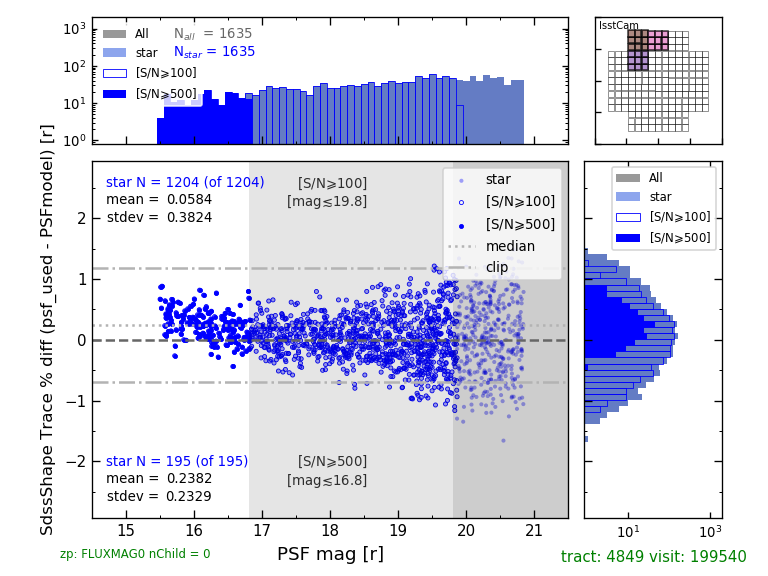
\includegraphics[width=0.8\textwidth]{plots/plot-v199540-psfTraceDiff-psfMagHist}
\caption{Brighter fatter effect evidence }
\label{fig:bfp}
\end{figure}



\subsubsection{Discussion}
We discussed how to implement change in code with tight turn around (need sign off from SciOps \gls{AD}).
How should one decide to rerun -  we need policies to affect or not nightly or daily changes in case of failures. Probably there is some percent level of problems we would accept, one percent seems ok two starts to seem a lot.  It was noted that problems stemming from a new software version should always have the possibility to revert to a previous stable version.

The need for some sort of rolled up \gls{QA} status were discussed - MacArthur came up with some summary files an example of which \texttt{visitAnalysis\_OpsRehearsal\_night1\_i.shortSum.txt} is in \appref{sec:visitsum}.


\subsection{Day 2} \label{sec:day2}

The daily meeting took place as planned at 11:00 \gls{PST}.

Transfers were initiated earlier than Day 1 with the 5 second delays removed, and all data had arrived at the \gls{LDF} by 7:30 am.
Data ingestion {\texttt{/project/OpsRehearsal\_1/night2} and processing were initiated shortly thereafter and were completed within roughly 1 hour.

No processing errors were reported, so examination of less severe issues were undertaken.
Noted were WARN-level problems that revolved around reference catalogs being in an outdated format
and the lack of zeropoint information for z- and Y-bands. 

\subsubsection{Discussion}
There were discussions about how the current \gls{pipeline}, operating on DC2 data might compare with what might
be needed during commissioning and operations.  
It was noted that because the rehearsal was using a processing \gls{pipeline} (and \gls{QA} tools) more amenable to \gls{Data Release Processing} (\gls{DRP}) that \gls{QA} products available might not be good comparisons to that needed when working with prompt processing.  
Also, it was noted that prompt processing \gls{QA} might form a basis for later selection of inputs to \gls{DRP}.

Another discussion revolved around whether WARN-level diagnostics might be dealt with in Operations/Commissioning.
Mostly it was felt that these fell into two classes:  those that were indicative of poor data (which might not require any intervention) and those that indicated software bugs (which should be tracked/resolved through tickets to the \gls{DM} developers).


\subsection{Day 3} \label{sec:day3}

The daily meeting took place as planned at 11:00 \gls{PST}.

Transfers were initiated similar to Day 2 and all data had arrived at the \gls{LDF} by 7:30 am.
Data ingestion {\texttt{/project/OpsRehearsal\_1/night3} required roughly 20 minutes.  
Processing was subsequently initiated but after 30 minutes it was found that jobs had never been submitte to the compute resource.  That resource (a reserved allocation) was found to still be running \gls{QA} from Night 2. An alternate compute resource was identified and jobs re-submitted, finishing $\sim$35 minutes later.

Similar WARN-level problems were identified prior to the daily meeting as were a 
small number of failures, similar to night 1 (number of stars resulting in failed \gls{PSF} modeling).

\subsubsection{Discussion}

Discussions centered on what information needed to be captured from this rehearsal for future rehearsals.
It was felt that this rehearsal proceeded relatively smoothly but did not include processes that could
mimic commissioning team's needs (i.e. fast turn around processing) and ad-hoc processing of data taken
to address specific tests.  The next rehearsal (late 2019/early 2020) is meant to focus toward 
LSST Commissioning with ComCam and should include Commissioning Team members.




\section{Conclusion and lessons learned}\label{sec:conc}
Though there were some limitations in out setup (\secref{sec:setup}) this was still useful exercise.

One central issue that should be followed-up on in subsequent rehearsals are the \gls{QA} metrics to be gathered during prompt processing and that utilities to provide rollups/summaries.

Though in the telecon status was discussed it was not properly recorded in the google sheet for the day,
there was no designated minute taker an individuals did not necessarily add a summary. In operations such a status
report should probably be filled even before the meeting.



